\documentclass[a4paper]{article}

\usepackage[utf8]{inputenc}
\usepackage[T1]{fontenc}

\usepackage{lmodern}
\usepackage{amsmath}
\usepackage{amssymb}
\usepackage{stmaryrd}

\usepackage{mathtools}
\usepackage{amsthm}
\usepackage{thmtools}
\declaretheorem{lemma}
\declaretheorem[style=definition,qed=$\blacktriangle$]{example}
\declaretheorem[style=definition,qed=$\blacktriangle$]{definition}
\numberwithin{equation}{section}

\usepackage{enumitem}
\setlist[enumerate,1]{label=\alph*)}
% FIXME use \newlist
\newenvironment{prfcases}{\begin{enumerate}[label={\it Case \arabic*.},leftmargin=0pt]}{\end{enumerate}}

\usepackage{algorithm}

\usepackage{tikz}
\usetikzlibrary{shapes.geometric}
\tikzset{itermtree/.style={anchor=north,child anchor=north,%
	level distance=6mm,sibling distance=10mm,%
	edge from parent/.style={draw,solid},every node/.style={solid}}}
\tikzset{pure/.style={draw,rectangle,inner sep=4pt,minimum size=5mm}}
\tikzset{term/.style={draw,circle,inner sep=1pt,minimum size=5mm}}
\tikzset{ap/.style={fill,diamond,inner sep=0pt,minimum size=6pt}}
\tikzset{subtrm/.style={draw,isosceles triangle,isosceles triangle apex angle=55,%
	shape border rotate=90,minimum height=10mm}}
\tikzset{abbrv/.style={dashed}}

\usepackage[
	style=numeric,
	sorting=none,
	doi=false,
	urldate=iso8601,
]{biblatex}
\addbibresource{bibliography.bib}

\usepackage[hidelinks]{hyperref}


\newcommand{\ldb}{\llbracket}
\newcommand{\rdb}{\rrbracket}
\newcommand{\todo}{\fbox{To do.}}

\newcommand{\oftype}{\mathrel{::}}
\newcommand{\funT}{\Rightarrow}
\newcommand{\abs}[2]{\lambda #1.\>#2}
\newcommand{\All}[2]{\bigwedge #1.\>#2}
\newcommand{\all}[2]{\forall #1.\>#2}
\newcommand{\set}[2]{\{#1\mid #2\}}

\DeclareMathOperator{\pure}{\mathit{pure}}
\newcommand{\ap}{\diamond}
\DeclareMathOperator{\sterm}{\mathsf{term}}
\DeclareMathOperator{\spure}{\mathsf{pure}}
\newcommand{\sap}{\mathbin{\mathsf{`ap`}}}
\newcommand{\sapp}{\>}
\newcommand{\sabs}[2]{{\boldsymbol\lambda} #1.\>#2}


\title{Applicative Functors in Isabelle/HOL: Notes}
\author{Joshua Schneider}

\begin{document}

\maketitle
\section{Project Overview}\label{sec:overview}

\subsection{Introduction}\label{subsec:introduction}

% TODO moved
Our primary goal is to implement an Isabelle/HOL proof method which reduces
lifted equations to their base form.
Here, lifting refers to a transition from operations on base types to related
operations on some structure.
Hinze~\cite{hinze10} studied the conditions under which lifting preserves the
validity of equations.
He noticed that lifting can be defined in an intuitive fashion if the target
structure is an applicative functor~\cite{mcbride08}:
a unary type constructor $f$ with associated constants%
\footnote{Types are given in Isabelle notation.}
\begin{align*}
	\pure_f &\oftype \alpha \funT \alpha f, \\
	(\ap_f) &\oftype (\alpha \funT \beta) f \funT \alpha f \funT \beta f.
\end{align*}
The operator $\ap_f$ is left-associative.
We omit the subscripts if the functor is clear from the context.
Moreover, the following laws must be satisfied:
\begin{align*}
	\tag{identity} \pure{\mathit{id}} \ap u &= u \\
	\tag{composition} \pure{(\cdot)} \ap u \ap v \ap w &= u \ap (v \ap w) \\
	\tag{homomorphism} \pure{f} \ap \pure x &= \pure{(f x)} \\
	\tag{interchange} u \ap \pure{x} &= \pure{(\abs{f}{f x})} \ap u
\end{align*}

The identity type constructor defined by $\alpha\,\mathit{id} = \alpha$ is a
trivial applicative functor for $\pure{x} = x$, $f \ap x = f x$.
We can take any abstraction-free term $t$ and replace each constant $c$ by
$\pure{c}$, and each instance of function application $f x$ by $f \ap x$.
The rewritten term is equivalent to $t$ under the identity functor
interpretation, or identity ``idiom'' as coined in \cite{mcbride08}.
By choosing a different applicative functor, we obtain a different
interpretation of the same term structure.
In fact, this is how we define the lifting of $t$ to an idiom.
We also permit variables, which remain as such in the lifted term, but range
over the structure instead.
A term consisting only of $\pure$ and $\ap$ applications and
free variables is called an idiomatic expression.

\begin{example}\label{exmp:set-intro}
Another applicative functor can be constructed from sets.
For each type $\alpha$ there is a corresponding type $\alpha\,\mathit{set}$
of sets with elements in $\alpha$;
$\pure$ denotes the singleton set constructor $x \mapsto \{x\}$;
$F \ap X$ takes a set of functions $F$ and a set of arguments $X$
with compatible type, applying each function to each argument:
\[ F \ap X = \set{f x}{f \in F,\, x \in X}. \]
We can lift addition on natural numbers to the set idiom by defining the operator
\begin{align*}
	(\oplus) &\oftype \mathit{nat}\,\mathit{set} \funT \mathit{nat}\,\mathit{set} \funT
		\mathit{nat}\,\mathit{set}, \\
	X \oplus Y &= \pure{(+)} \ap X \ap Y = \set{x + y}{x \in X,\, y \in Y}.
\end{align*}
The associative property of addition
\[ \all{x y z}{(x + y) + z = x + (y + z)} \]
can be translated to sets of natural numbers
\[ \all{X Y Z}{(X \oplus Y) \oplus Z = X \oplus (Y \oplus Z)}, \]
where it holds as well, as one can check with a slightly laborious proof.
Note that the two sides of the latter equation are the lifted counterparts
of the former, respectively.
\end{example}

As we have seen, lifting can be generalized to equations.
There is actually a more fundamental relationship between the two equations
from above example---the lifted form can be proven for all applicative
functors, not just $\mathit{set}$, using only the base property and the
applicative functor laws.
We want to automate this step with a proof method.

Not all equations can be lifted in all idioms, though.
Stronger conditions are required if the list of quantified variables is
different for each side of the equation.
(The left-to-right order is relevant, but not the nesting within the terms.)
These conditions must basically ensure that the functor does not add ``too many
effects'' which go beyond the simple embedding of a base type.
Such effects may be evoked if a variable takes an impure value, i.e., a value
which is not equal to $\pure x$ for any $x$.

\begin{example}\label{exmp:set-counterexmp}
We try to lift the fact that zero is a left absorbing element for
multiplication of integers, $\all{x \oftype \mathit{int}}{0 \cdot x = 0}$,
to sets.
Note that the variable $x$ occurs only on the left.
But the lifted equation does not hold: If $x$, now generalized to
$\mathit{int}\,\mathit{set}$, is instantiated with the empty set, then
\[ \pure{(\cdot)} \ap \pure 0 \ap \{\} = \{\} \ne \pure 0. \]
Here the effect of $\{\}$ is that it cancels out everything else if it occurs
somewhere in an idiomatic expression.
This makes it impossible to lift any equation with a variable occuring only on
one side to $\mathit{set}$.
\end{example}

\section{Normal Form Conversion}\label{sec:normal-form}

McBride and Paterson~\cite{mcbride08} noted that idiomatic expressions can
be transformed into an application of a pure function to a sequence of impure
arguments.
Hinze~\cite{hinze10} gave an explicit construction of this normal form for the
monoidal variant of applicative functors.
The normal form is useful for our purpose because the pure part reflects the
term that was lifted.
Its construction can be performed using only the applicative laws, so this is
the most general approach regarding instances (but not regarding lifted
equalities).
In the following, we define lifting and normalization formally, based on a
syntactic representation of idiomatic terms.
Then we describe the implementation of the normalization procedure in
Isabelle/ML.

\subsection{The Idiomatic Calculus}\label{subsec:idiomatic-calculus}

In Section~\ref{subsec:introduction}, we introduced idiomatic expressions built
from $\pure$ and $\ap$ constants of an applicative functor.
This structure maps straightforward to a recursive datatype, given that there
is a representation for arguments of $\pure$.
These must have a some structure as well such that the applicative laws can
be expressed.
It should also be possible to have ``opaque'' idiomatic subterms, which cannot
(or should not) be written as a combination of $\pure$ and $\ap$.
This is primarily useful for variables ranging over lifted types, but as
demonstrated in Example~\ref{exmp:set-usage}, more complex terms may occur too.
Therefore it makes sense to refer to general lambda terms in both cases;
then we can define semantics consistently.
However, types are ignored for simplicity.

\begin{definition}[Untyped lambda terms]
Let $\mathcal{V}$ be an infinite set of variable symbols.
We assume that $f$, $g$, $x$, $y$ are disjoint variables.
The set of untyped lambda terms is defined as
\begin{equation}
	\mathcal{T} ::= \mathcal{V} \mid (\mathcal{T} \sapp \mathcal{T}) \mid
		\sabs{\mathcal{V}}{\mathcal{T}}
\end{equation}
An equivalence relation on $\mathcal{T}$ is a $\mathcal{T}$-congruence iff it
is closed under application and abstraction.
Let $\termeq$ be the smallest $\mathcal{T}$-congruence containing $\alpha$-,
$\beta$-, and $\eta$-conversion.
\end{definition}

\begin{definition}[Idiomatic terms]
The set of idiomatic terms is defined as
\begin{equation}
	\mathcal{I} ::= \sterm \mathcal{T} \mid \spure \mathcal{T} \mid
		\mathcal{I} \sap \mathcal{I}.
\end{equation}
$\sap$ associates to the left.
An $\mathcal{I}$-congruence is an equivalence relation closed under $\sap$.
The congruence $\simeq$ is induced by the rules
\begin{align}
	x &\simeq \spure{(\sabs{x}{x})} \sap x \label{eq:iterm-id}\\
	g \sap (f \sap x) &\simeq \spure \mathbf{B} \sap g \sap f \sap x \label{eq:iterm-comp}\\
	\spure f \sap \spure x &\simeq \spure (f \sapp x) \label{eq:iterm-morph}\\
	f \sap \spure x &\simeq \spure{((\sabs{x}\sabs{f}{f \sapp x}) \sapp x)} \sap f \label{eq:iterm-xchng}
\end{align}
where $\mathbf{B}$ abbreviates
$\mathbf{B} = \sabs{g}{\sabs{f}{\sabs{x}{g \sapp (f \sapp x)}}}$.
\end{definition}

$\sterm$ represents arbitrary values in the lifted domain, whereas $\spure$
lifts a value.
The introduction rules for the relation $\simeq$ are obviously the syntactical
counterparts of the applicative laws.
Together with symmetry, substitution, etc., they give rise to a simple
calculus of equivalence judgements.
The intuitive meaning of $s \simeq t$ is that the terms can be used
interchangeably.
For example, there is a derivation for
\begin{equation}\label{eq:pure-rotate}
	\spure g \sap (f \sap x) \simeq \spure{(\mathbf{B} \sapp g)} \sap f \sap x
\end{equation}
from \eqref{eq:iterm-comp}, where $g$ is instantied with $\spure g$, and a
substitution along \eqref{eq:iterm-morph} on the right-hand side.

\begin{figure}
\begin{minipage}[t]{0.46\textwidth}\centering
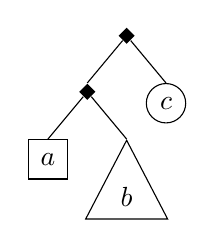
\begin{tikzpicture}[itermtree]
	\node[ap] {} child {
		node[ap] {} child { node[pure] {$a$} } child[subtrm] { node[subtrm] {$b$} }
	} child { node[term] {$c$} };
\end{tikzpicture}
\caption{$(\spure a \sap b) \sap \sterm c$ as a tree.}
\label{fig:iterm-ex}
\end{minipage}\hfill
\begin{minipage}[t]{0.46\textwidth}\centering
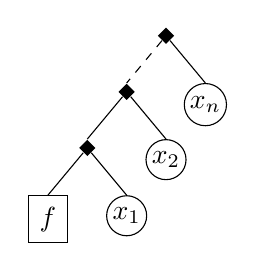
\begin{tikzpicture}[itermtree]
	\node[ap] {} child {
		node[ap] {} child {
			node[ap] {} child {
				node[pure] {$f$}
			} child { node[term] {$x_1$} }
		} child { node[term] {$x_2$} }
	    edge from parent [abbrv]
	} child { node[term] {$x_n$} };
\end{tikzpicture}
\caption{A term in normal form.}
\label{fig:iterm-nf-ex}
\end{minipage}
\end{figure}

Idiomatic terms are visualized naturally as trees.
This will be helpful in explaining term transformations.
Figure~\ref{fig:iterm-ex} shows the conventions:
Inner nodes correspond to $\sap$, leaves are either pure terms (boxes) or
opaque terms (circles).
Whole subterms may be abbreviated by a triangle.
A term has normal form if it consists of a single pure node to which a number
of opaque terms (or none) are applied in sequence.
Figure~\ref{fig:iterm-nf-ex} gives a general example.
A formal construction follows:

\begin{definition}[Normal form]
The set $\mathcal{N} \subset \mathcal{I}$ of idiomatic terms in normal form is
defined inductively as
\begin{gather}
	\spure x \in \mathcal{N}, \label{eq:nf-base}\\
	t \in \mathcal{N} \implies t \sap \sterm s \in \mathcal{N}. \label{eq:nf-step}
\end{gather}
\end{definition}

\begin{figure}\centering
\begin{tikzpicture}[itermtree]
	\node[ap] {} child { node[pure] {$g$} } child {
		node[ap] {} child[subtrmn] { node[subtrm] {$t'$} } child { node[term] {$x$} }
	};
\end{tikzpicture}
\raisebox{10mm}{$\qquad\simeq\qquad$}
\begin{tikzpicture}[itermtree]
	\node[ap] {} child {
		node[ap] {} child {
			node[ap] {} child { node[pure] {$\mathbf{B}$} } child { node[pure] {$g$} }
		} child[subtrmf] { node[subtrm] {$t'$} }
	} child { node[term] {$x$} };
\end{tikzpicture}
\raisebox{10mm}{$\qquad\simeq\qquad$}
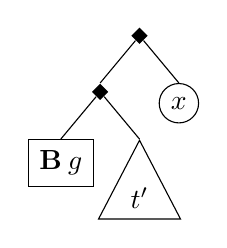
\begin{tikzpicture}[itermtree]
	\node[ap] {} child {
		node[ap] {} child { node[pure] {$\mathbf{B} \sapp g$} } child[subtrm] { node[subtrm] {$t'$} }
	} child { node[term] {$x$} };
\end{tikzpicture}
\caption{The ``pure-rotate'' step.}
\label{fig:pure-rotate}
\end{figure}

It is not entirely obvious how the normal form can be derived from equations
\eqref{eq:iterm-id}--\eqref{eq:iterm-xchng}.
Rewriting blindly with these is prone to infinite recursion.
Therefore we need a more controlled algorithm.
Consider an idiomatic term $t$.
If $t$ is a single pure term, then it is already in normal form.
The case $t = \sterm x$ is also easy:
Due to \eqref{eq:iterm-id}, we have $t \simeq \spure{(\sabs{x}{x})} \sap t$,
which is in normal form.
But in the case of $t = u \sap v$, various steps could be performed,
depending on the subterms.
We simplify the situation by normalizing each subterm recursively, so we get
an equivalent term $u' \sap v'$ where $u',v' \in \mathcal{N}$.

Now let us assume that $u'$ is just $\spure g$.
If $v'$ is also a pure term, they can be combined along \eqref{eq:iterm-morph}.
Otherwise, the term looks like the one on the left of Figure~\ref{fig:pure-rotate}.
As is shown there, the term tree can be rotated such that one opaque term moves
to the outer-most level.
This is the same equivalence as stated in \eqref{eq:pure-rotate}.
Because the remaining part again has the shape ``pure term applied to normal
form'', we proceed recursively.
In pattern-matching style, the transformation `pure-nf' reads
\begin{align}
	\operatorname{pure-nf}(\spure g \sap (f \sap x)) &=
		\operatorname{pure-nf}{(\spure{(\mathbf{B} g)} \sap f)} \sap x \\
	\operatorname{pure-nf}(\spure f \sap \spure x) &= \spure{(f x)}
\end{align}
\begin{lemma}\label{thm:pure-nf}
For all $g \in \mathcal{T}$ and $t \in \mathcal{N}$,
$\operatorname{pure-nf}(\spure g \sap t)$ is well-defined, and%
\/\footnote{$a \in S \simeq b$ abbreviates ``$a \in S$ and $a \simeq b$''.}
$\operatorname{pure-nf}(\spure g \sap t) \in \mathcal{N} \simeq \spure g \sap t$.
\end{lemma}
\begin{proof}
We prove all claims simultaneously by induction on $t \in \mathcal{N}$,
where $g$ is arbitrary.
\begin{prfcases}
\item Assume $t = \spure x$ for some $x \in \mathcal{T}$.
	Only the second equation applies, so we have
	\[ \operatorname{pure-nf}(\spure g \sap t) = \spure{(g \sapp x)}. \]
	All pure terms are in $\mathcal{N}$, and equivalence follows from
	\eqref{eq:iterm-morph}.
\item Assume $t = t' \sap \sterm x$ for some
	$t' \in \mathcal{N}$, $x \in \mathcal{T}$, and that the hypothesis holds
	for $t'$ and all $g$.
	Only the first equation applies, so
	\[ \operatorname{pure-nf}(\spure g \sap t) =
		\operatorname{pure-nf}(\spure{(\mathbf{B} g)} \sap t') \sap \sterm x. \]
	Instantiating the induction hypothesis, we find that
	\[ \operatorname{pure-nf}(\spure{(\mathbf{B} \sapp g)} \sap t') \in \mathcal{N} \simeq
		\spure{(\mathbf{B} \sapp g)} \sap t' \]
	is well-defined.
	$\mathcal{N}$ is closed under application to opaque terms \eqref{eq:nf-step},
	hence $\operatorname{pure-nf}(\spure g \sap t) \in \mathcal{N}$.
	Finally, we have
	\begin{align*}
		\operatorname{pure-nf}(\spure g \sap t) &\simeq
			\spure{(\mathbf{B} \sapp g)} \sap t' \sap \sterm x \\
		&\stackrel{\mathclap{\eqref{eq:pure-rotate}}}{\simeq}
			\spure g \sap (\spure t' \sap \sterm x) =
			\spure g \sap t. \qedhere
	\end{align*}
\end{prfcases}
\end{proof}

Going back to $u' \sap v'$, we assumed that $u'$ is a pure term.
The case where $v'$ is pure instead can be translated to the former by
\begin{equation}
	\operatorname{nf-pure}(f \sap \spure x) =
		\operatorname{pure-nf}{(\spure{((\sabs{x}\sabs{f}{f x}) \sapp x)} \sap f)} \\
\end{equation}
\begin{lemma}\label{thm:nf-pure}
For all $t \in \mathcal{N}$ and $x \in \mathcal{T}$,
$\operatorname{nf-pure}(t \sap \spure x)$ is well-defined, and
$\operatorname{nf-pure}(t \sap \spure x) \in \mathcal{N} \simeq t \sap \spure x$.
\end{lemma}
\begin{proof}
Follows from Lemma~\ref{thm:pure-nf} and \eqref{eq:iterm-xchng}.
\end{proof}

\begin{figure}\centering
\begin{tikzpicture}[itermtree]
	\node[ap] {} child[subtrmf] { node[subtrm] {$s$} } child {
		node[ap] {} child[subtrmn] { node[subtrm] {$t'$} } child { node[term] {$x$} }
	};
\end{tikzpicture}
\raisebox{10mm}{$\qquad\simeq\qquad$}
\begin{tikzpicture}[itermtree]
	\node[ap] {} child {
		node[ap] {} child {
			node[ap] {} child { node[pure] {$\mathbf{B}$} } child[subtrmn] {
				node[subtrm] {$s$}
			}
		} child[subtrmf] { node[subtrm] {$t'$} }
	} child { node[term] {$x$} };
\end{tikzpicture}
\caption{The ``rotate'' step.}
\label{fig:rotate}
\end{figure}

Finally, we look at general $u'$, $v'$.
A term rotation is useful again, see Figure~\ref{fig:rotate}.
Before recursion, we must normalize the subterm $\spure \mathbf{B} \sap s$.
But we already know how to do this: by `pure-nf'.
The base case is reached when $v'$ is a single pure term, which is the domain
of `nf-pure'.
The corresponding transformation is therefore
\begin{align}
	\operatorname{nf-nf}(g \sap (f \sap x)) &=
		\operatorname{nf-nf}{(\operatorname{pure-nf}{(\spure \mathbf{B} \sap g)} \sap f)} \sap x \\
	\operatorname{nf-nf}(t) &= \operatorname{nf-pure}(t) \quad\text{(otherwise)}
\end{align}
\begin{lemma}\label{thm:nf-nf}
For all $s,t \in \mathcal{N}$, 
$\operatorname{nf-nf}(s \sap t)$ is well-defined, and
$\operatorname{nf-nf}(s \sap t) \in \mathcal{N} \simeq s \sap t$.
\end{lemma}
\begin{proof}
The proof is similar to the one of Lemma~\ref{thm:pure-nf}, by induction on
$t \in \mathcal{N}$ and arbitrary $s \in \mathcal{N}$.
\begin{prfcases}
\item Assume $t = \spure x$ for some $x \in \mathcal{T}$.
	The second equation applies, so we have
	\[ \operatorname{nf-nf}(s \sap t) = \operatorname{nf-pure}(s \sap \spure x). \]
	Since $s \in \mathcal{N}$, the claim follows directly from Lemma~\ref{thm:nf-pure}.
\item Assume $t = t' \sap \sterm x$ for some
	$t' \in \mathcal{N}$, $x \in \mathcal{T}$, and that the hypothesis holds
	for $t'$ and all $s \in \mathcal{N}$.
	Only the first equation applies,
	\[ \operatorname{nf-nf}(s \sap t) =
		\operatorname{nf-nf} (\operatorname{pure-nf}(\spure \mathbf{B} \sap s) \sap t') \sap \sterm x. \]
	We have
	$\operatorname{pure-nf}(\spure \mathbf{B} \sap s) \in \mathcal{N} \simeq \spure \mathbf{B} \sap s$
	from Lemma~\ref{thm:pure-nf}.
	Thus we can instantiate the induction hypothesis, and the transformed term
	is indeed in normal form.
	Furthermore,
	\begin{align*}
		\operatorname{nf-nf}(s \sap t) &\stackrel{\mathclap{\text{(IH)}}}{\simeq}
			\operatorname{pure-nf}(\spure \mathbf{B} \sap s) \sap t' \sap \sterm x \\
		&\simeq \spure \mathbf{B} \sap s \sap t' \sap \sterm x \\
		&\stackrel{\mathclap{\eqref{eq:iterm-comp}}}{\simeq}
			s \sap (t' \sap \sterm x) = s \sap t. \qedhere
	\end{align*}
\end{prfcases}
\end{proof}

\begin{algorithm}[t]
\caption{Normalization of idiomatic terms.}
\label{alg:normalize}
\begin{gather*}
	\begin{align*}
		\operatorname{normalize}(\spure x) &= \spure x \\
		\operatorname{normalize}(\sterm x) &= \spure{(\sabs{x}{x})} \sap \sterm x \\
		\operatorname{normalize}(x \sap y) &=
			\operatorname{nf-nf}(\operatorname{normalize} x \sap \operatorname{normalize} y)
	\end{align*} \\[2ex]
	\begin{align*}
		\operatorname{nf-nf}(g \sap (f \sap x)) &=
			\operatorname{nf-nf}{(\operatorname{pure-nf}{(\spure \mathbf{B} \sap g)} \sap f)} \sap x \\
		\operatorname{nf-nf}(t) &= \operatorname{nf-pure}(t) \quad\text{(otherwise)}
	\end{align*} \\[2ex]
	\begin{align*}
		\operatorname{pure-nf}(\spure g \sap (f \sap x)) &=
			\operatorname{pure-nf}{(\spure{(\mathbf{B} g)} \sap f)} \sap x \\
		\operatorname{pure-nf}(\spure f \sap \spure x) &= \spure{(f x)}
	\end{align*} \\[2ex]
	\operatorname{nf-pure}(f \sap \spure x) =
		\operatorname{pure-nf}{(\spure{((\sabs{x}\sabs{f}{f x}) \sapp x)} \sap f)}
\end{gather*}
\end{algorithm}

Algorithm~\ref{alg:normalize} summarizes all pieces of the normal form
transformation.
`normalize' is the entry point and performs the main recursion mentioned in the
beginning.
We haven't proved the desired property for `normalize' yet, but this is just a
straightforward induction.

\begin{lemma}\label{thm:normalize}
For all $t \in \mathcal{I}$, $\operatorname{normalize} t$ is well-defined, and
$\operatorname{normalize} t \in \mathcal{N} \simeq t$.
\end{lemma}
\begin{proof}
By induction on $t$, Lemma~\ref{thm:nf-nf}, and equation \eqref{eq:iterm-id}.
\end{proof}

Until now, we only have considered the syntactic structure of idiomatic terms
together with the artificial relation $\simeq$, which is also based on syntax.
In order to define the semantics of idiomatic terms, we assume that we operate
in an equational theory $\Omega$ based on $\mathcal{T}$-terms, where
$=_\Omega\,\supseteq\,\termeq$ is an equivalence relation.

\begin{definition}[Idiomatic interpretation]\label{def:iterm-interp}
Let $\iota = \langle p, a \rangle$ with $p,a \in \mathcal{T}$.
The interpretation $\ldb t \rdb_\iota$ of the idiomatic term $t$ w.r.t. $\iota$
is defined as
\begin{align}
	\ldb \sterm t \rdb_\iota &= t, \\
	\ldb \spure t \rdb_\iota &= p \sapp t, \\
	\ldb s \sap t \rdb_\iota &= (a \sapp \ldb s \rdb_\iota) \sapp \ldb t \rdb_\iota.
\end{align}
$\iota$ is an idiomatic structure (in $\Omega$) iff
\begin{equation}
	\all{q r}{q \simeq r \implies \ldb q \rdb_\iota =_\Omega \ldb r \rdb_\iota}.
\end{equation}
\end{definition}

\begin{definition}\label{def:id-structure}
\begin{equation}
	\iota_\mathrm{id} = \langle \sabs{x}{x}, \sabs{f}{\sabs{x}{f \sapp x}} \rangle
\end{equation}
is the identity structure.
\end{definition}

% TODO lift \termeq to I

\begin{lemma}\label{thm:normal-form}
For all $t \in \mathcal{I}$, there is a unique term $t' \in \mathcal{N}$ such
that $t \simeq t'$.
\end{lemma}
\begin{proof}
Existence of the normal form is a corollary of Lemma~\ref{thm:normalize}.
In order to show that it is unique, we construct a relation
$R \subseteq \mathcal{I}\times\mathcal{I}$, such that
\begin{itemize}
\item for all idiomatic terms $s$ and $t$, $s \simeq t \implies (s,t) \in R$, and
\item for all terms in normal form $n$ and $n'$, $(n,n') \in R \implies n \termeq n'$.
\end{itemize}
$R$ is defined in two steps.
The first deals with the sequence of opaque terms,
\[
	\operatorname{opaq}(\spure x) = [], \quad
	\operatorname{opaq}(\sterm x) = [x], \quad
	\operatorname{opaq}(s \sap t) = \operatorname{opaq}(s) @ \operatorname{opaq}(t).
\]
Let $(s,t) \in R'$ if and only if $\operatorname{opaq}(s) = \operatorname{opaq}(t)$
pointwise.
Now assume $(s,t) \in R'$.
We can modify both terms such that all opaque terms are replaced by new pure
variables, say $\spure v_1,\dots,\spure v_n$.
The mapping is the same for both terms, i.e., the variable is determined by
the position in $\operatorname{opaq}(\_)$.
Let $s'$, $t'$ be these modified terms.
Then $(s,t) \in R$ if and only if
$\ldb s' \rdb_{\iota_\mathrm{id}} \termeq \ldb t' \rdb_{\iota_\mathrm{id}}$.

It remains to show that $R$ satisfies both properties.
\todo
\end{proof}

\begin{lemma}
\todo\ Every encoding of an applicative functor in $\Omega$ is an idiomatic
structure.
Especially $\iota_\mathrm{id}$ is an idiomatic structure.
\end{lemma}

\begin{definition}[Lifted terms]
$q \in \mathcal{I}$ is a lifting of $t \in \mathcal{T}$ if 
$\ldb q \rdb_{\iota_\mathrm{id}} =_\Omega t$.
\end{definition}

\begin{lemma}
Let $q$ be a lifting of $t$. The normal form $q'$ of $q$ can be written as
\[ q' = ( \cdots ((\spure t' \sap \sterm a_1) \sap \sterm a_2) \cdots ) \sap \sterm a_n. \]
Then $t' \sapp \vec a =_\Omega t$.
\end{lemma}
\todo

\printbibliography

\end{document}
